\documentclass[aspectratio=169]{beamer}

\usetheme{Madrid}
\usecolortheme{seahorse}
\setbeamertemplate{navigation symbols}{}
\setbeamertemplate{footline}{}
\usepackage{booktabs}
\usepackage{graphicx}
\hypersetup{bookmarks=false}

\title[Event-State Forecasting]{Leakage-Aware Deep Learning for Financial Event-State Forecasting}
\author{Jose Ignacio Valdivia Aguero}
\institute{University of Luxembourg}
\date{DL Course Project}

\begin{document}

\begin{frame}
  \titlepage
  \vspace{-0.5em}
  \centering\small Multi-horizon excess-return forecasting with leakage-aware deep-learning benchmarks.
\end{frame}

\begin{frame}{Talk Roadmap}
\begin{columns}[T]
\begin{column}{0.48\textwidth}
\textbf{Question}
\begin{itemize}
  \item Can aligned company-news event states improve multi-horizon excess-return forecasts?
  \item Can deep models help without leaking future information?
\end{itemize}
\end{column}
\begin{column}{0.48\textwidth}
\textbf{Answer}
\begin{itemize}
  \item XGBoost is the strongest lockbox RMSE/MAE forecaster.
  \item TSMixer is the strongest lockbox portfolio-ranking model.
  \item The main contribution is a rigorous, reproducible forecasting system.
\end{itemize}
\end{column}
\end{columns}
\end{frame}

\begin{frame}{Why This Is Hard}
\begin{columns}[T]
\begin{column}{0.55\textwidth}
\begin{itemize}
  \item Returns have low signal-to-noise and strong nonstationarity.
  \item News can matter, but timestamps, no-news days, and provider truncation create hidden biases.
  \item Model selection can overfit validation folds even when deep models look plausible.
\end{itemize}
\end{column}
\begin{column}{0.42\textwidth}
\begin{block}{Design principle}
Train/validation is for search. Lockbox is the final excess-return forecasting test.
\end{block}
\begin{block}{Metric principle}
ROC-AUC is not applicable: this is continuous excess-return regression.
\end{block}
\end{column}
\end{columns}
\end{frame}

\begin{frame}{Protocol: Leakage-Aware Artifact Pipeline}
\begin{center}
\small
\begin{tabular}{@{}llll@{}}
\toprule
Stage & Artifact & Key control & Output \\
\midrule
Data & Top-50 + OHLCV + news & no raw overwrite & row universe \\
Features & market + event states & no-news rows preserved & sidecars \\
Splits & expanding folds + lockbox & purge/embargo & split manifest \\
Training & fold-local preprocessing & no lockbox tuning & saved preds \\
Evaluation & RMSE/MAE + rank IC & bootstrap + lockbox & reports \\
\bottomrule
\end{tabular}
\end{center}
\vspace{0.5em}
\begin{itemize}
  \item Horizons: 1d, 5d, 10d, 20d, 60d.
  \item Lockbox ends 2026-02-13; all result roots keep manifests and prediction packets.
\end{itemize}
\end{frame}

\begin{frame}{State of the Art Context}
\begin{columns}[T]
\begin{column}{0.50\textwidth}
\textbf{Financial ML baselines}
\begin{itemize}
  \item Efficient-market discipline and expected-return multiple testing.
  \item Gradient boosting is still a very strong tabular baseline.
  \item Forecast metrics: RMSE, MAE, OOS $R^2$, rank IC.
\end{itemize}
\end{column}
\begin{column}{0.48\textwidth}
\textbf{Deep learning candidates}
\begin{itemize}
  \item FinBERT/BERT for semantic financial text features.
  \item TSMixer and Transformer-family sequence models.
  \item PatchTST, iTransformer, TFT, and Chronos motivate richer temporal architectures.
\end{itemize}
\end{column}
\end{columns}
\end{frame}

\begin{frame}{Implemented Model Stack}
\begin{columns}[T]
\begin{column}{0.33\textwidth}
\textbf{Text/Event}
\begin{itemize}
  \item Alpha Vantage aligned news.
  \item No-news as explicit state.
  \item FinBERT sidecars for later fusion.
\end{itemize}
\end{column}
\begin{column}{0.33\textwidth}
\textbf{Market}
\begin{itemize}
  \item Lag/rolling features.
  \item Linear and fixed XGBoost baselines.
  \item XGBoost: 800-trial tuned baseline.
\end{itemize}
\end{column}
\begin{column}{0.30\textwidth}
\textbf{Sequence/Mixer}
\begin{itemize}
  \item TSMixer sequence models.
  \item Readout correction audit.
  \item Mixed model: frozen-base horizon mixer.
\end{itemize}
\end{column}
\end{columns}
\end{frame}

\begin{frame}{Tuning Trace: Search Was Auditable}
\begin{center}
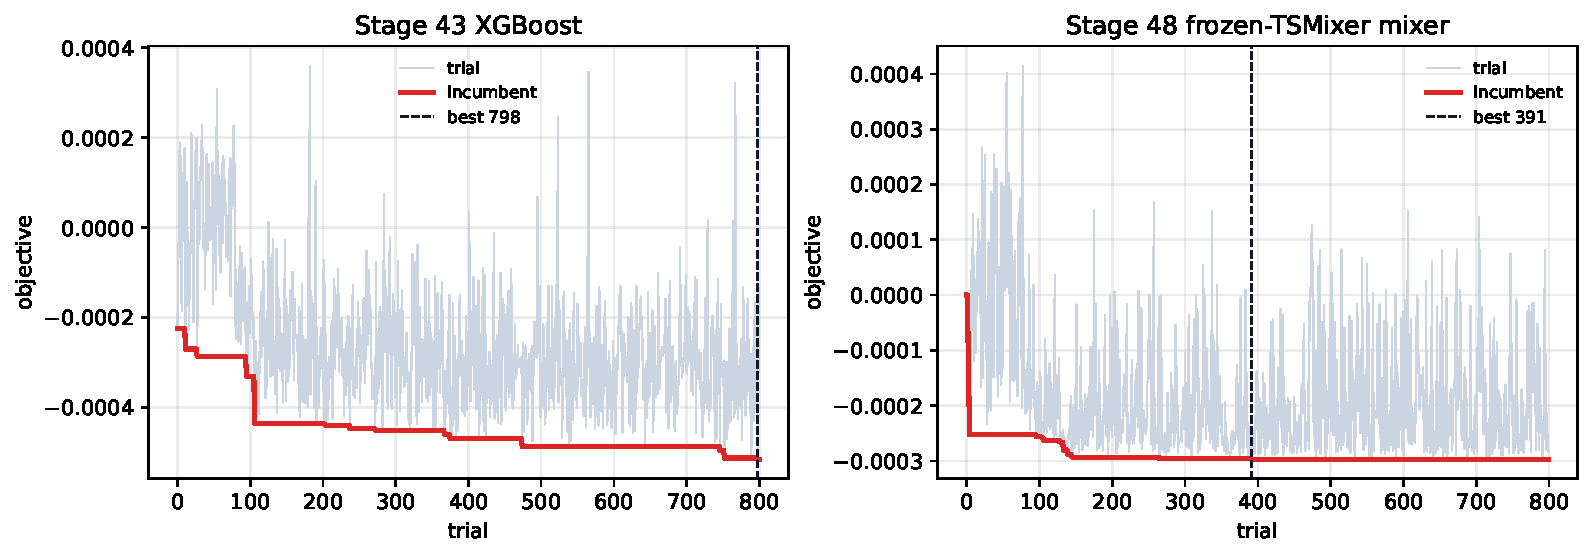
\includegraphics[width=0.95\textwidth]{report_artifacts/tuning_curves.pdf}
\end{center}
\vspace{-0.5em}
\begin{itemize}
  \item XGBoost Optuna search completed 800 trials; selected model wins lockbox RMSE/MAE.
  \item Mixed model completed 800 meta/mixer trials; validation gains did not beat XGBoost error on lockbox.
  \item Both searches used zero lockbox rows for tuning.
\end{itemize}
\end{frame}

\begin{frame}{Exact Lockbox RMSE by Horizon}
\begin{center}
\small
\begin{tabular}{@{}lrrrr@{}}
\toprule
Horizon & XGBoost & TSMixer & Mixed model & Best \\
\midrule
1d & 0.0214 & 0.0221 & 0.0214 & XGBoost \\
5d & 0.0468 & 0.0469 & 0.0469 & XGBoost \\
10d & 0.0661 & 0.0670 & 0.0665 & XGBoost \\
20d & 0.0943 & 0.0949 & 0.0944 & XGBoost \\
60d & 0.1929 & 0.1972 & 0.1942 & XGBoost \\
\bottomrule
\end{tabular}
\end{center}
\vspace{0.4em}
\begin{itemize}
  \item Error increases sharply with horizon, as expected for longer excess-return windows.
  \item XGBoost is the most consistent lockbox error-metric model.
\end{itemize}
\end{frame}

\begin{frame}{Primary Metrics: Lockbox RMSE and MAE}
\begin{center}
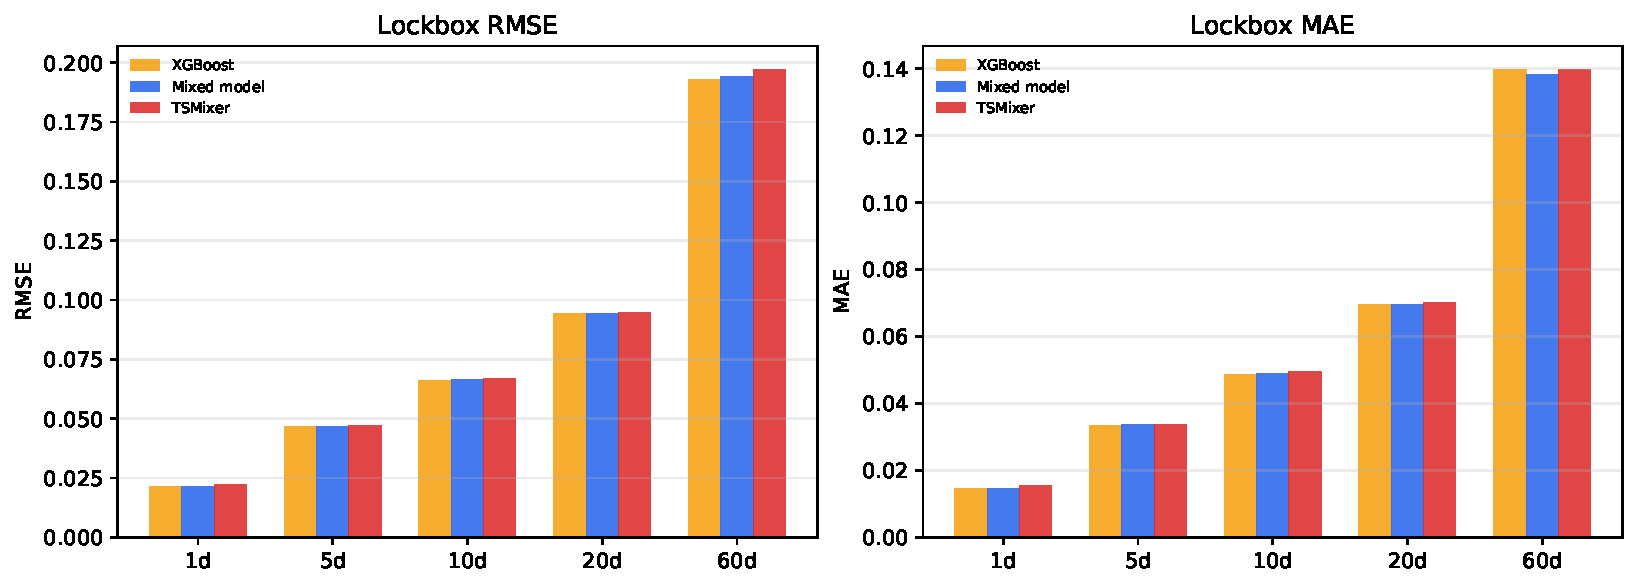
\includegraphics[width=0.95\textwidth]{report_artifacts/lockbox_rmse_mae.pdf}
\end{center}
\vspace{-0.5em}
\begin{itemize}
  \item Regression metrics are primary because labels are continuous forward excess returns.
  \item XGBoost gives the strongest lockbox RMSE profile across horizons.
\end{itemize}
\end{frame}

\begin{frame}{Error Winner vs Ranking Winner}
\begin{center}
\small
\begin{tabular}{@{}lll@{}}
\toprule
Question & Winner & Evidence \\
\midrule
Lowest lockbox RMSE/MAE & XGBoost & best RMSE across all 5 horizons \\
Best lockbox portfolio simulation & TSMixer & 15.05\%, \$115,045 over 137 days \\
Best Mixed model role & validation fusion & validation delta $-2.97\times10^{-4}$ vs XGB \\
Mixed lockbox error vs XGB & XGBoost & Mixed delta $+9.20\times10^{-5}$ \\
Main interpretation & objective matters & calibrated error and ranking diverge \\
\bottomrule
\end{tabular}
\end{center}
\vspace{0.4em}
\begin{itemize}
  \item XGBoost learned the most accurate excess-return levels under RMSE/MAE.
  \item TSMixer produced the strongest cross-sectional ranking signal in portfolio simulation.
\end{itemize}
\end{frame}

\begin{frame}{Secondary Evidence: Ranking and Uncertainty}
\begin{center}
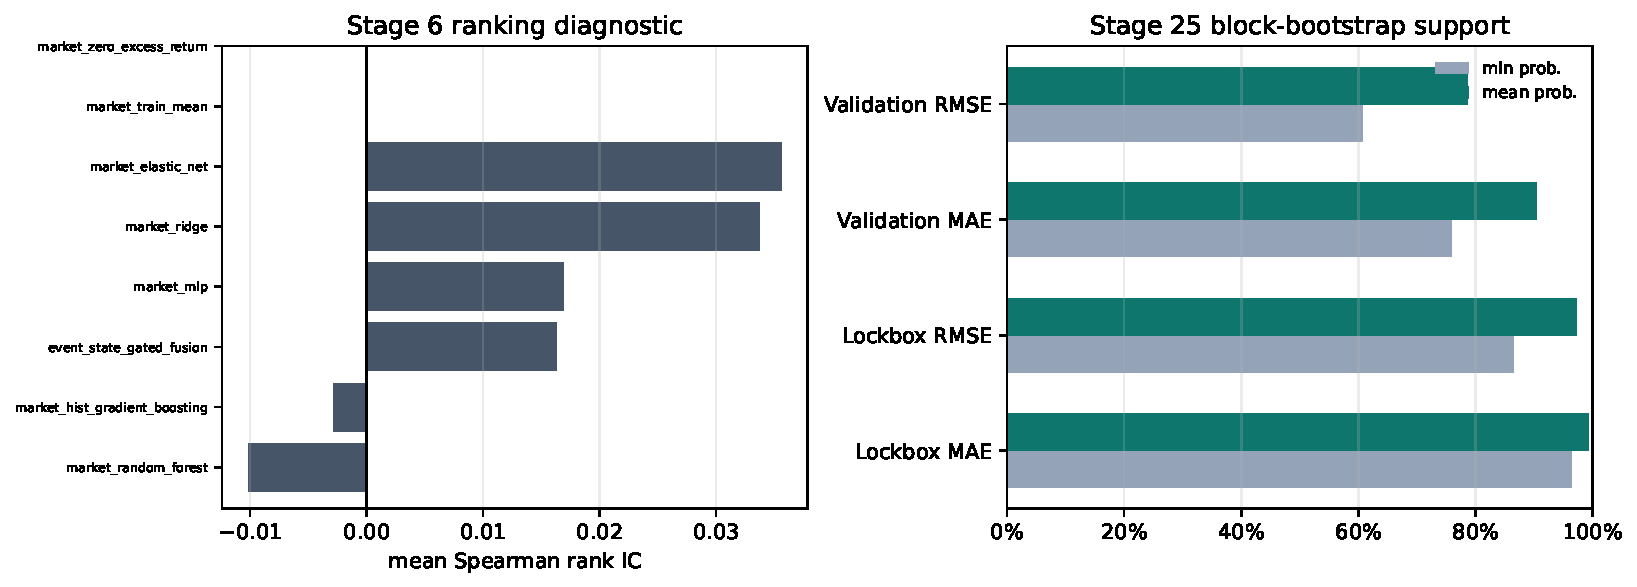
\includegraphics[width=0.92\textwidth]{report_artifacts/ranking_uncertainty.pdf}
\end{center}
\vspace{-0.5em}
\begin{itemize}
  \item Rank IC and hit-rate results describe cross-sectional forecast quality.
  \item Moving-block bootstrap checks temporal dependence and uncertainty.
\end{itemize}
\end{frame}

\begin{frame}{Lockbox Portfolio Simulation}
\begin{center}
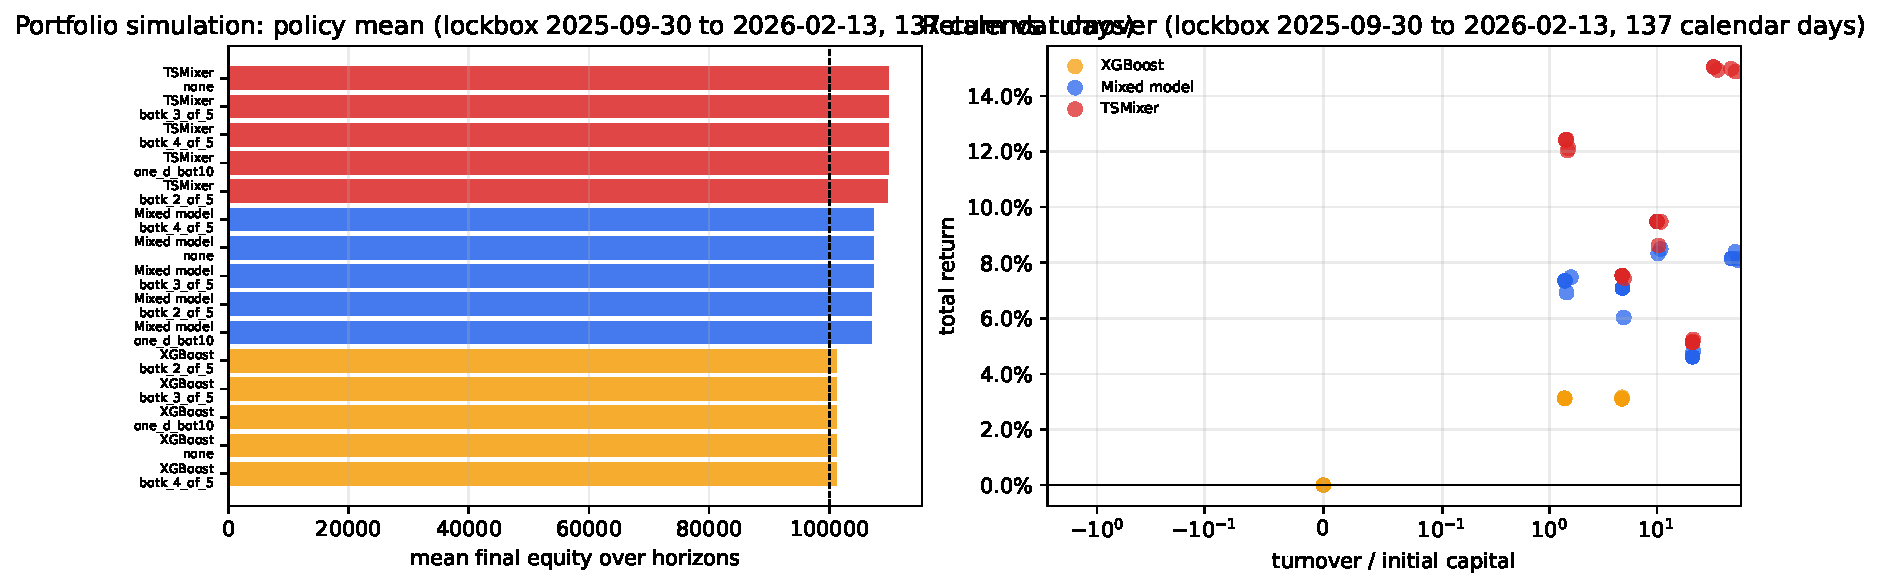
\includegraphics[width=0.82\textwidth]{report_artifacts/portfolio_simulations.pdf}
\end{center}
\vspace{-0.5em}
\begin{itemize}
  \item Initial capital: \$100k; long-only, fractional shares, no costs, no slippage, no taxes.
  \item Lockbox trading window: 2025-09-30 to 2026-02-13, 137 calendar days, about 4.5 months.
  \item Best row: \$115,045 final equity; it uses frozen TSMixer sequence predictions.
  \item XGBoost short-horizon no-trade cases identify flat-rank signal construction for the next model.
\end{itemize}
\end{frame}

\begin{frame}{Portfolio Bar Charts by Horizon}
\begin{center}
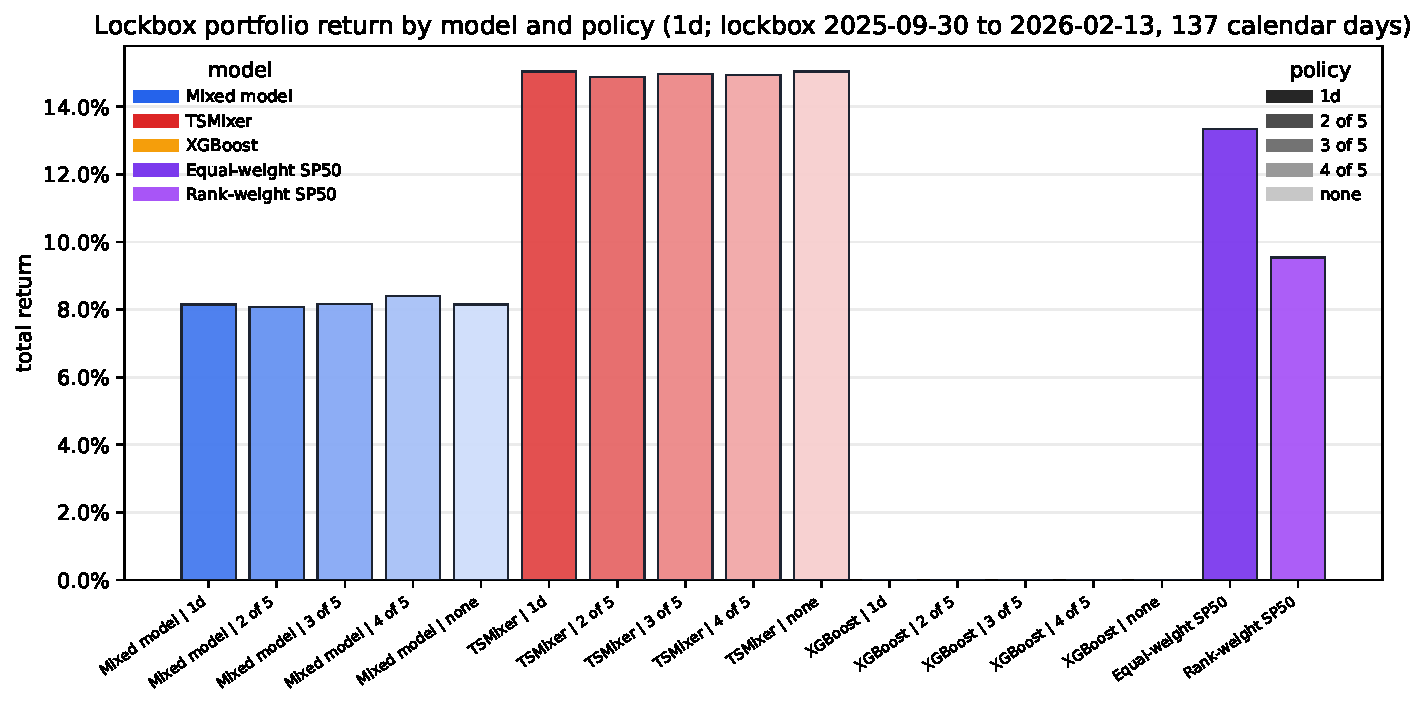
\includegraphics[width=0.31\textwidth]{report_artifacts/portfolio_returns_by_policy_model_1d.pdf}
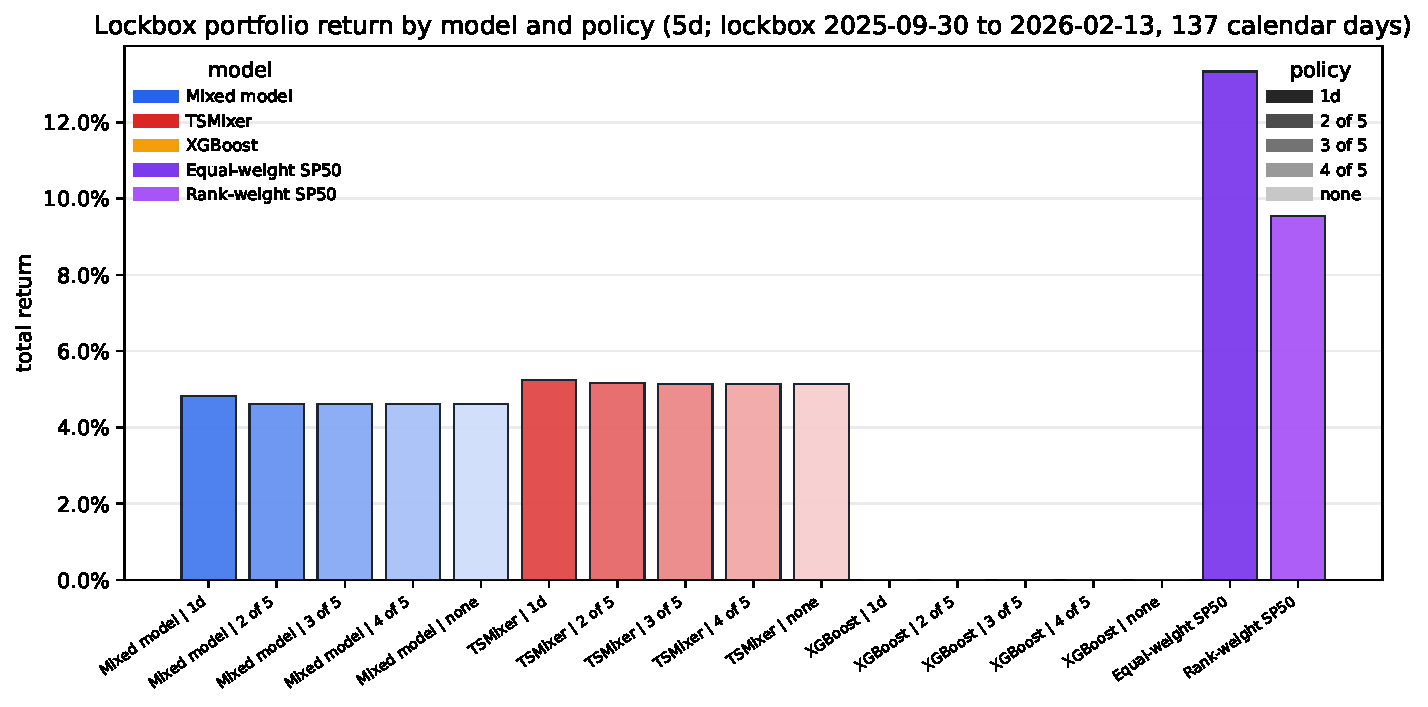
\includegraphics[width=0.31\textwidth]{report_artifacts/portfolio_returns_by_policy_model_5d.pdf}
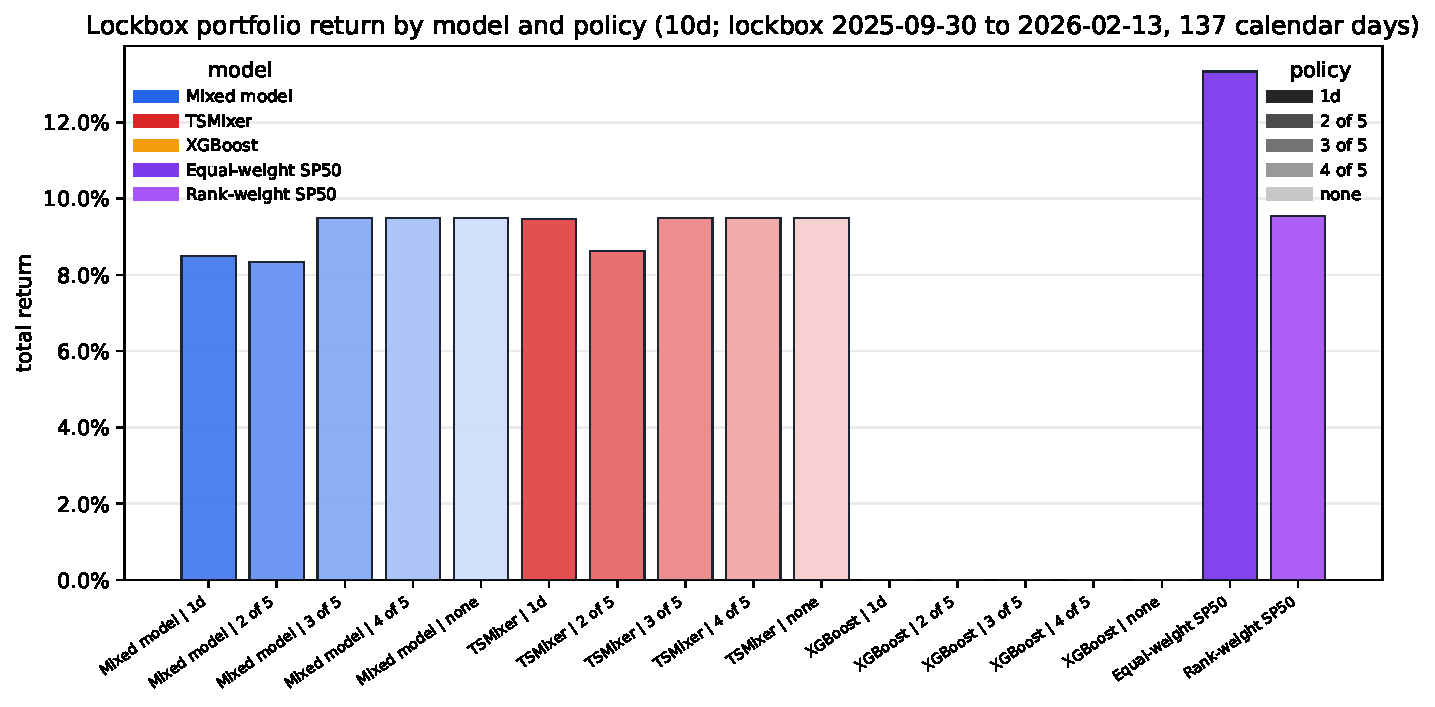
\includegraphics[width=0.31\textwidth]{report_artifacts/portfolio_returns_by_policy_model_10d.pdf}
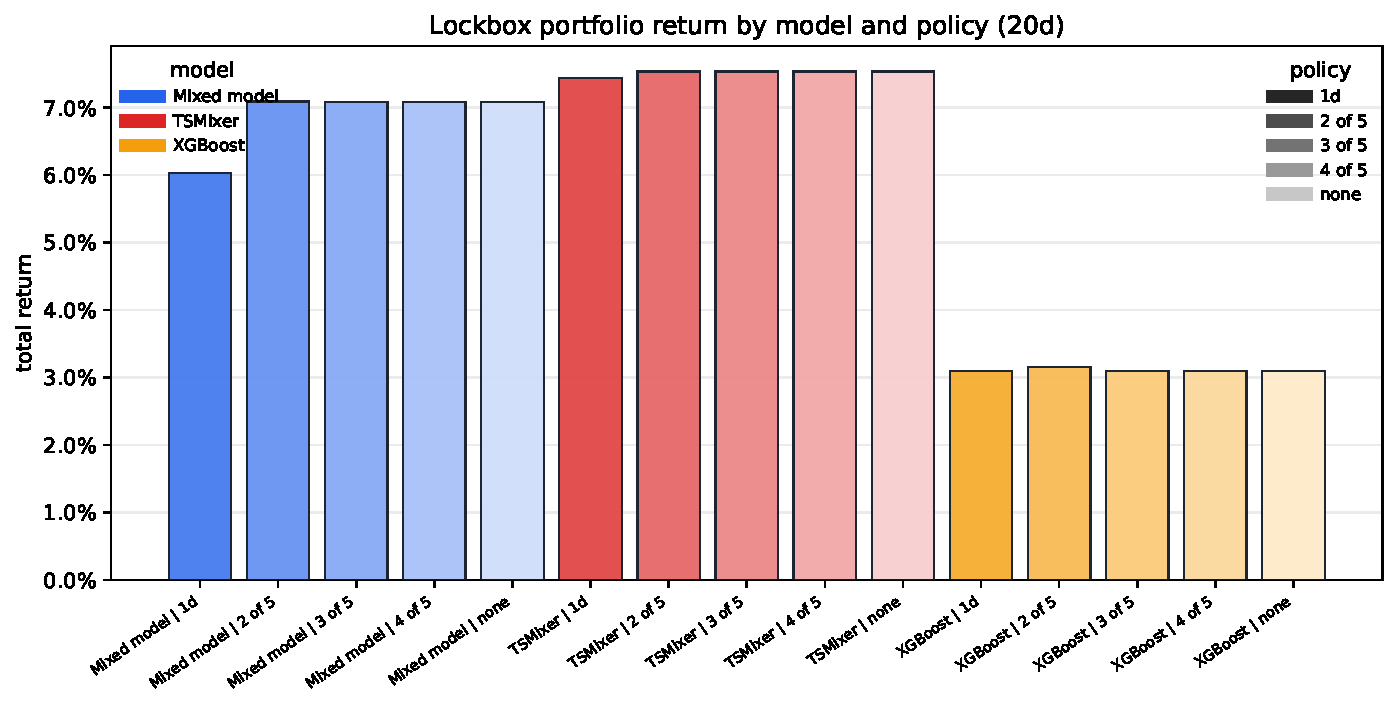
\includegraphics[width=0.31\textwidth]{report_artifacts/portfolio_returns_by_policy_model_20d.pdf}
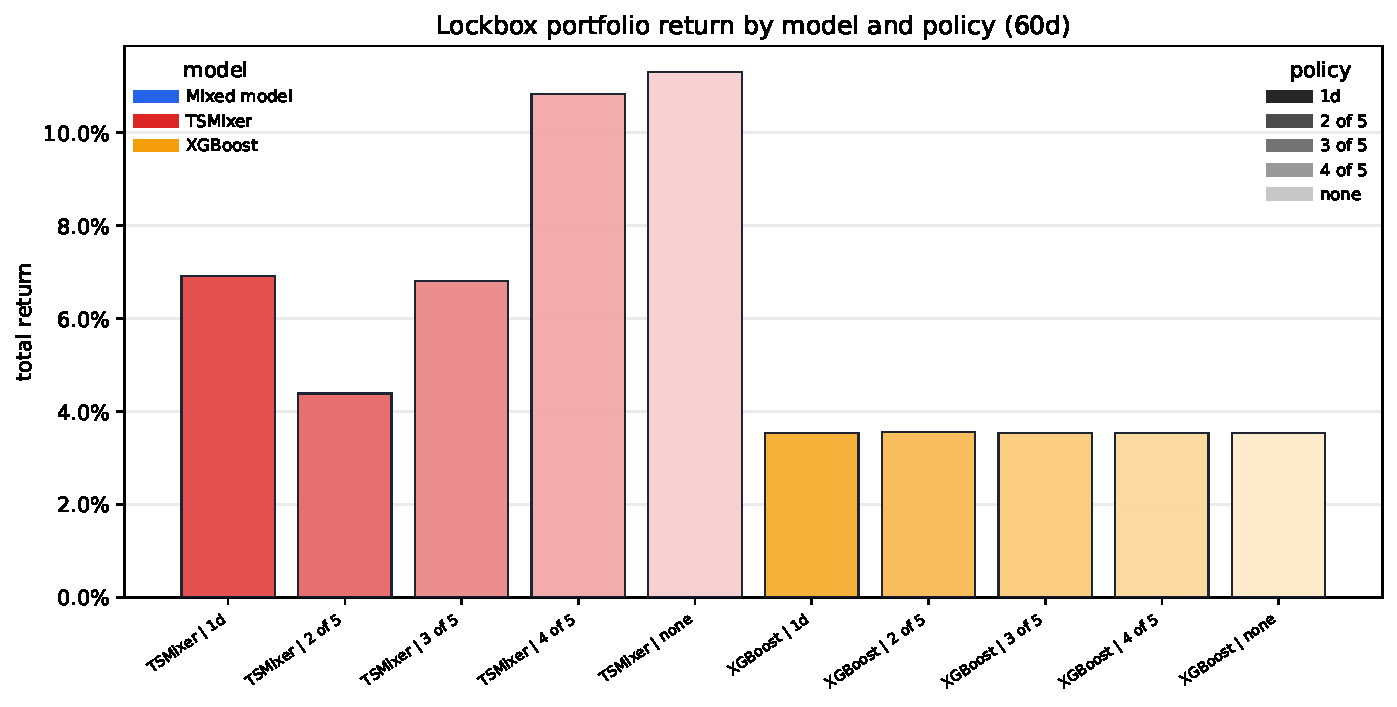
\includegraphics[width=0.31\textwidth]{report_artifacts/portfolio_returns_by_policy_model_60d.pdf}
\end{center}
\vspace{-0.6em}
\begin{itemize}
  \item Bars include model-policy simulations plus Equal-weight SP50 and Rank-weight SP50 proxies.
  \item The 15.05\% top row is over 137 calendar days, not a long annual test.
\end{itemize}
\end{frame}

\begin{frame}{Main Numerical Results}
\begin{center}
\small
\begin{tabular}{@{}lll@{}}
\toprule
Evidence & Result & Interpretation \\
\midrule
XGBoost lockbox delta & $-5.34\times10^{-4}$ vs prior XGB & best error forecaster \\
XGBoost both-metric rate & 62.2\% & consistent error improvement \\
TSMixer best portfolio row & 15.05\%, \$115,045 & best ranking simulation \\
Mixed validation delta & $-2.97\times10^{-4}$ vs XGB & looked useful in search \\
Mixed lockbox delta & $+9.20\times10^{-5}$ vs XGB & fusion did not beat XGBoost error \\
ROC-AUC & not reported & continuous regression target \\
\bottomrule
\end{tabular}
\end{center}
\end{frame}

\begin{frame}{How Good Is the Final Model?}
\begin{center}
\small
\begin{tabular}{@{}lll@{}}
\toprule
Dimension & Judgment & Evidence \\
\midrule
Error forecasting & XGBoost leads & best RMSE across all horizons \\
Relative error gain & measurable & XGBoost delta $-5.34\times10^{-4}$ \\
Ranking simulation & TSMixer leads & 15.05\% top row over 137 days \\
Mixed model value & useful validation fusion & $-2.97\times10^{-4}$ validation delta \\
Model-selection lesson & objective-specific winner & error and ranking diverge \\
Research value & strong & leakage-aware artifacts and audits \\
\bottomrule
\end{tabular}
\end{center}
\end{frame}

\begin{frame}{Discussion: What I Learned}
\begin{columns}[T]
\begin{column}{0.50\textwidth}
\textbf{Positive lessons}
\begin{itemize}
  \item Reproducibility can be engineered through manifests, saved predictions, and tests.
  \item Tree baselines are hard to beat in small financial tabular settings.
  \item Deep sequence models need architecture audits and strong baselines; high validation score does not automatically translate to lockbox performance.
\end{itemize}
\end{column}
\begin{column}{0.48\textwidth}
\textbf{Next steps}
\begin{itemize}
  \item Try a deeper reinforcement learning model with capacity to rank predictions from most probable to least probable.
  \item Expand data collection beyond API limits with a reproducible scraping/cache layer.
  \item Add transaction costs and slippage before any portfolio-style interpretation.
\end{itemize}
\end{column}
\end{columns}
\end{frame}

\begin{frame}{Final Conclusion}
\begin{block}{Scientific conclusion}
XGBoost is the final strongest lockbox error forecaster; TSMixer is the strongest lockbox ranking-simulation model.
\end{block}
\begin{block}{Deep learning conclusion}
For financial forecasting, the most important DL competence is not just adding BERT, TSMixer, or Transformers; it is controlling leakage, validating architecture semantics, and resisting overfit narratives.
\end{block}
\begin{block}{Performance and simulation conclusion}
Performance gains are measurable across the lockbox: XGBoost improves calibrated excess-return error, while TSMixer gives the best realized portfolio-ranking simulation at 15.05\% over 137 calendar days.
\end{block}
\end{frame}

\begin{frame}
  \centering
  \vspace{2.2em}
  {\LARGE THANK YOU}
\end{frame}

\end{document}
